\documentclass[aspectratio=169]{beamer}

% Standard Beamer/AMS/TikZ tools only.
\usepackage{amsmath}
\usepackage{tikz}

\usetheme{Madrid}
\usecolortheme{seahorse}

\newcommand{\R}{\mathbb{R}}
\newcommand{\grad}{\nabla}
\newcommand{\inner}[2]{\left\langle #1,#2\right\rangle}
\newcommand{\Lagr}{\mathcal{L}}
\newcommand{\act}{\mathcal{A}}

\title{The Karush-Kuhn-Tucker Theorem}
\subtitle{Optimality conditions, proof sketch, and examples}
\author{}
\date{}

\begin{document}

\begin{frame}
  \titlepage
  \vspace{-1em}
  \begin{center}
    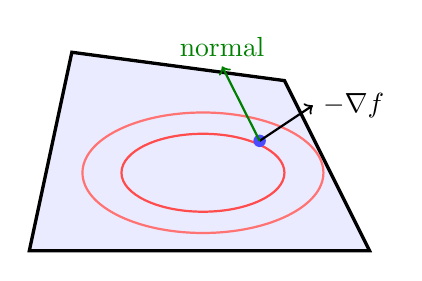
\begin{tikzpicture}[scale=.9]
      \draw[very thick,fill=blue!8] (0,0) -- (4.8,0) -- (3.6,2.4) -- (.6,2.8) -- cycle;
      \draw[thick,red!70] (2.45,1.1) ellipse (1.15 and .55);
      \draw[thick,red!55] (2.45,1.1) ellipse (1.7 and .85);
      \fill[blue!70] (3.25,1.55) circle (2.5pt);
      \draw[->,thick] (3.25,1.55) -- (4.0,2.05) node[right] {$-\nabla f$};
      \draw[->,thick,green!50!black] (3.25,1.55) -- (2.72,2.60) node[above] {normal};
    \end{tikzpicture}
  \end{center}
\end{frame}

\begin{frame}{Why KKT conditions matter}
  \begin{columns}[T,totalwidth=\textwidth]
  \begin{column}{.55\textwidth}
    KKT conditions turn a constrained optimization problem into algebraic equations and inequalities.
    \vspace{.5em}
    \begin{itemize}
      \item They generalize ``gradient equals zero.''
      \item Multipliers measure marginal value of constraints.
      \item In convex problems, they often certify global optimality.
      \item In algorithms, they define residuals and stopping tests.
    \end{itemize}
  \end{column}
  \begin{column}{.42\textwidth}
    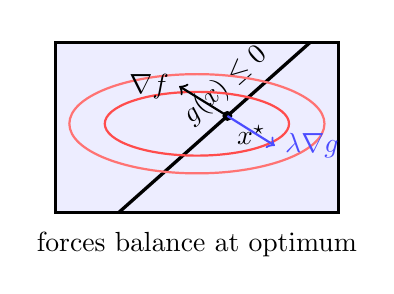
\begin{tikzpicture}[scale=.9]
      \draw[very thick,fill=blue!7] (0,0) rectangle (4,2.4);
      \draw[very thick] (.9,0) -- (3.6,2.4) node[pos=.64,above,sloped] {$g(x)\le 0$};
      \draw[red!70,thick] (2.0,1.25) ellipse (1.3 and .45);
      \draw[red!55,thick] (2.0,1.25) ellipse (1.8 and .7);
      \fill (2.43,1.36) circle (2pt) node[below right] {$x^\star$};
      \draw[->,thick] (2.43,1.36) -- (1.75,1.78) node[left] {$\nabla f$};
      \draw[->,thick,blue!70] (2.43,1.36) -- (3.10,.94) node[right] {$\lambda\nabla g$};
      \node at (2,-.45) {forces balance at optimum};
    \end{tikzpicture}
  \end{column}
  \end{columns}
\end{frame}

\begin{frame}{Problem form and notation}
  We consider the nonlinear program
  \[
    \begin{array}{ll}
      \text{minimize} & f(x) \\
      \text{subject to} & g_i(x)\le 0,\quad i=1,\ldots,m,\\
                        & h_j(x)=0,\quad j=1,\ldots,p,
    \end{array}
    \qquad x\in\R^n .
  \]
  \vspace{.3em}
  At a feasible point $x$, the active set is
  \[
    \act(x)=\{i: g_i(x)=0\}.
  \]
  \vspace{.3em}
  The Lagrangian is
  \[
    \Lagr(x,\lambda,\nu)=f(x)+\sum_{i=1}^m\lambda_i g_i(x)+\sum_{j=1}^p\nu_j h_j(x).
  \]
  The multipliers $\lambda_i$ are constrained by signs; the $\nu_j$ are free.
\end{frame}

\begin{frame}{The KKT conditions}
  A triple $(x^\star,\lambda^\star,\nu^\star)$ satisfies KKT if
  \begin{align*}
    &\text{stationarity:} &
      \nabla f(x^\star)+\sum_{i=1}^m\lambda_i^\star\nabla g_i(x^\star)+\sum_{j=1}^p\nu_j^\star\nabla h_j(x^\star)&=0,\\
    &\text{primal feasibility:} &
      g_i(x^\star)\le 0,\quad h_j(x^\star)&=0,\\
    &\text{dual feasibility:} &
      \lambda_i^\star&\ge 0,\\
    &\text{complementarity:} &
      \lambda_i^\star g_i(x^\star)&=0.
  \end{align*}
  \vspace{.4em}
  Complementarity says: each inequality is either active and priced, or inactive and unpriced.
\end{frame}

\begin{frame}{Geometry: gradient balance at a boundary optimum}
  \begin{columns}[T,totalwidth=\textwidth]
  \begin{column}{.45\textwidth}
    If only one inequality is active, stationarity reads
    \[
      \nabla f(x^\star)+\lambda^\star\nabla g(x^\star)=0,
      \qquad \lambda^\star\ge 0.
    \]
    Thus $-\nabla f(x^\star)$ lies in the normal cone generated by active constraints.
  \end{column}
  \begin{column}{.52\textwidth}
    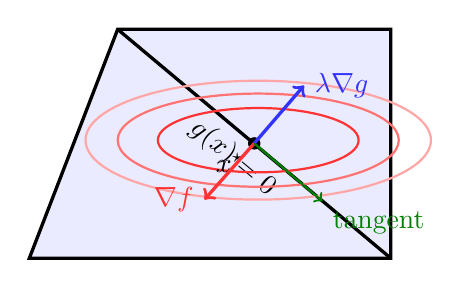
\begin{tikzpicture}[scale=1.02]
      \draw[very thick,fill=blue!8] (-.1,-.05) -- (4.4,-.05) -- (4.4,2.8) -- (1.0,2.8) -- cycle;
      \draw[very thick] (1.0,2.8) -- (4.4,-.05) node[pos=.48,below,sloped] {$g(x)=0$};
      \draw[red!80,thick] (2.75,1.42) ellipse (1.25 and .40);
      \draw[red!55,thick] (2.75,1.42) ellipse (1.75 and .58);
      \draw[red!35,thick] (2.75,1.42) ellipse (2.15 and .74);
      \fill[black] (2.70,1.38) circle (2.2pt) node[below left] {$x^\star$};
      \draw[->,very thick,red!80] (2.70,1.38) -- (2.08,.68) node[left] {$\nabla f$};
      \draw[->,very thick,blue!80] (2.70,1.38) -- (3.32,2.10) node[right] {$\lambda\nabla g$};
      \draw[->,thick,green!50!black] (2.70,1.38) -- (3.55,.66) node[below right] {tangent};
    \end{tikzpicture}
  \end{column}
  \end{columns}
\end{frame}

\begin{frame}{The theorem: necessary conditions}
  \begin{block}{KKT theorem, necessary form}
  Suppose $f,g_i,h_j$ are continuously differentiable near a local minimizer $x^\star$. If a constraint qualification holds at $x^\star$, then there exist multipliers $\lambda^\star\in\R^m$ and $\nu^\star\in\R^p$ satisfying the KKT conditions.
  \end{block}
  \vspace{.5em}
  Common constraint qualifications:
  \begin{itemize}
    \item LICQ: gradients of active inequalities and equalities are linearly independent.
    \item MFCQ: equality gradients are independent and there is a feasible first-order direction strictly decreasing all active inequalities.
    \item Slater's condition in convex optimization: there is a point satisfying all affine equalities and all convex inequalities strictly.
  \end{itemize}
\end{frame}

\begin{frame}{The theorem: sufficient conditions}
  \begin{block}{KKT theorem, convex sufficiency}
  Assume $f$ and $g_i$ are convex, and $h_j$ are affine. If a feasible point $x^\star$ has multipliers satisfying KKT, then $x^\star$ is a global minimizer.
  \end{block}
  \vspace{.6em}
  Proof in one line. For any feasible $x$,
  \begin{align*}
    f(x)&\ge f(x^\star)+\nabla f(x^\star)^T(x-x^\star)\\
        &=f(x^\star)-\sum_i\lambda_i^\star \nabla g_i(x^\star)^T(x-x^\star)
          -\sum_j\nu_j^\star \nabla h_j(x^\star)^T(x-x^\star)\\
        &\ge f(x^\star)-\sum_i\lambda_i^\star\bigl(g_i(x)-g_i(x^\star)\bigr)=f(x^\star)-\sum_i\lambda_i^\star g_i(x)\ge f(x^\star).
  \end{align*}
\end{frame}

\begin{frame}{Proof sketch for necessity: feasible directions}
  At a local minimizer, no first-order feasible direction can decrease $f$.
  \vspace{.3em}
  \[
    \nabla f(x^\star)^Td \ge 0
  \]
  for every direction $d$ satisfying the linearized constraints
  \[
    \nabla g_i(x^\star)^Td\le 0\quad (i\in\act),
    \qquad \nabla h_j(x^\star)^Td=0.
  \]
  \vspace{.4em}
  Under a constraint qualification, the linearized cone correctly approximates feasible first-order motion.

  \begin{center}
  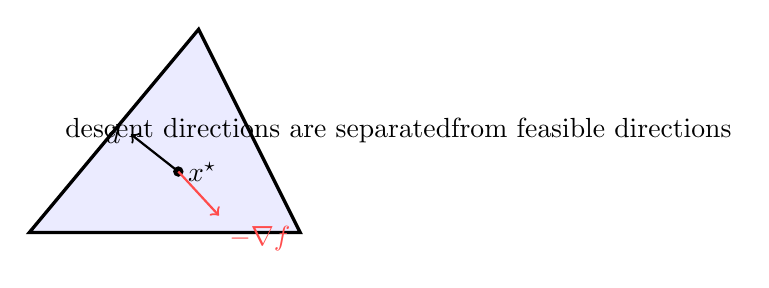
\begin{tikzpicture}[scale=.86]
    \fill[blue!8] (0,0) -- (4,0) -- (2.5,3) -- cycle;
    \draw[very thick] (0,0)--(4,0)--(2.5,3)--cycle;
    \fill (2.2,.9) circle (2.2pt) node[right] {$x^\star$};
    \draw[->,thick] (2.2,.9)--(1.5,1.45) node[left] {$d$};
    \draw[->,thick,red!70] (2.2,.9)--(2.8,.25) node[below right] {$-\nabla f$};
    \node at (5.45,1.5) {descent directions are separated\par from feasible directions};
  \end{tikzpicture}
  \end{center}
\end{frame}

\begin{frame}{Proof sketch for necessity: Farkas/separation}
  The previous slide says the system
  \[
    \nabla f(x^\star)^Td<0,\quad
    \nabla g_i(x^\star)^Td\le 0\ (i\in\act),\quad
    \nabla h_j(x^\star)^Td=0
  \]
  has no solution.
  \vspace{.3em}

  By a theorem of alternatives, this is equivalent to the existence of multipliers with
  \[
    \nabla f(x^\star)+\sum_{i\in\act}\lambda_i\nabla g_i(x^\star)+\sum_j\nu_j\nabla h_j(x^\star)=0,
    \qquad \lambda_i\ge 0.
  \]
  Set $\lambda_i=0$ for inactive constraints. Then complementarity follows automatically.
  \vspace{.5em}

  \begin{center}
  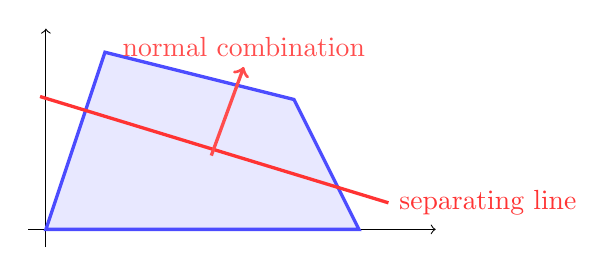
\begin{tikzpicture}[scale=.75]
    \draw[->] (-.3,0)--(6.6,0);
    \draw[->] (0,-.3)--(0,3.4);
    \fill[blue!9] (0,0)--(5.3,0)--(4.2,2.2)--(1,3)--cycle;
    \draw[very thick,blue!70] (0,0)--(5.3,0)--(4.2,2.2)--(1,3)--cycle;
    \draw[very thick,red!80] (-.1,2.25)--(5.8,.45) node[right] {separating line};
    \draw[->,very thick,red!70] (2.8,1.25)--(3.35,2.75) node[above] {normal combination};
  \end{tikzpicture}
  \end{center}
\end{frame}

\begin{frame}{Economic meaning of multipliers}
  Consider a parameterized constraint $g_i(x)\le b_i$.
  Under regularity, the optimal value $v(b)$ often satisfies
  \[
    \frac{\partial v}{\partial b_i}=-\lambda_i^\star
  \]
  for the sign convention $g_i(x)-b_i\le 0$.
  \vspace{.5em}
  Interpretation:
  \begin{itemize}
    \item Active constraints can have positive prices.
    \item Inactive constraints have zero price.
    \item A larger $\lambda_i$ means relaxing the constraint gives a larger first-order improvement.
  \end{itemize}
  \vspace{.3em}
  This is why KKT multipliers are also called shadow prices.
\end{frame}

\begin{frame}{Example 1: equality constrained least squares}
  \[
    \min_x \; \frac12\|Ax-b\|^2
    \quad \text{subject to}\quad Cx=d.
  \]
  Lagrangian:
  \[
    \Lagr(x,\nu)=\frac12\|Ax-b\|^2+\nu^T(Cx-d).
  \]
  KKT conditions:
  \[
    A^T(Ax-b)+C^T\nu=0,
    \qquad Cx=d.
  \]
  Equivalently,
  \[
    \begin{bmatrix}
      A^TA & C^T\\
      C & 0
    \end{bmatrix}
    \begin{bmatrix}x\\ \nu\end{bmatrix}
    =
    \begin{bmatrix}A^Tb\\ d\end{bmatrix}.
  \]
  A constrained optimization problem becomes a structured linear system.
\end{frame}

\begin{frame}{Example 2: projection onto a halfspace}
  Project $y\in\R^n$ onto $\{x:a^Tx\le b\}$:
  \[
    \min_x \frac12\|x-y\|^2\quad\text{s.t.}\quad a^Tx-b\le 0.
  \]
  KKT gives
  \[
    x-y+\lambda a=0,\qquad \lambda\ge0,
    \quad a^Tx\le b,
    \quad \lambda(a^Tx-b)=0.
  \]
  Therefore
  \[
    x^\star=y-\lambda a,
    \qquad
    \lambda=\max\left\{0,\frac{a^Ty-b}{\|a\|^2}\right\}.
  \]
  \begin{center}
  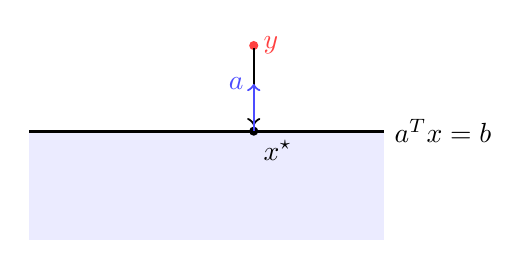
\begin{tikzpicture}[scale=.75]
    \fill[blue!8] (-3,-1.2)--(3,-1.2)--(3,.65)--(-3,.65)--cycle;
    \draw[very thick] (-3,.65)--(3,.65) node[right] {$a^Tx=b$};
    \fill[red!75] (.8,2.1) circle (2.2pt) node[right] {$y$};
    \fill[black] (.8,.65) circle (2.2pt) node[below right] {$x^\star$};
    \draw[->,thick] (.8,2.05)--(.8,.75);
    \draw[->,thick,blue!70] (.8,.65)--(.8,1.45) node[left] {$a$};
  \end{tikzpicture}
  \end{center}
\end{frame}

\begin{frame}{Example 3: a simple bound-constrained quadratic}
  \[
    \min_x \frac12(x-c)^2\quad\text{s.t.}\quad x\ge 0.
  \]
  Write the constraint as $g(x)=-x\le0$. The KKT conditions are
  \[
    x-c-\lambda=0,
    \qquad x\ge0,
    \qquad \lambda\ge0,
    \qquad \lambda x=0.
  \]
  Hence
  \[
    x^\star=\max\{c,0\},
    \qquad
    \lambda^\star=\max\{-c,0\}.
  \]
  \vspace{.3em}
  \begin{columns}[T,totalwidth=\textwidth]
  \begin{column}{.48\textwidth}
  If $c>0$, the unconstrained minimizer is feasible and $\lambda=0$.
  \end{column}
  \begin{column}{.48\textwidth}
  If $c<0$, the bound is active and $\lambda=-c$ pushes the solution to $0$.
  \end{column}
  \end{columns}
\end{frame}

\begin{frame}{Example 4: water filling / resource allocation}
  Allocate resource $x_i\ge0$ with budget $\sum_i x_i=P$:
  \[
    \max_{x_i\ge0}\sum_{i=1}^n \log(\alpha_i+x_i)
    \quad\text{s.t.}\quad \sum_i x_i=P.
  \]
  Equivalently minimize the negative objective. KKT gives, for $x_i>0$,
  \[
    \frac{1}{\alpha_i+x_i}=\mu,
    \qquad\text{so}\qquad x_i=\frac1\mu-\alpha_i.
  \]
  Including nonnegativity,
  \[
    x_i^\star=\max\{0,\tau-\alpha_i\},
    \qquad \sum_i x_i^\star=P.
  \]
  \begin{center}
  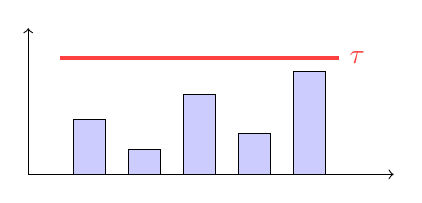
\begin{tikzpicture}[scale=.58]
    \draw[->] (0,0)--(8,0);
    \draw[->] (0,0)--(0,3.2);
    \foreach \x/\h in {1/1.2,2.2/.55,3.4/1.75,4.6/.9,5.8/2.25}
      {\draw[fill=blue!20] (\x,0) rectangle +(0.7,\h);}
    \draw[very thick,red!75] (.7,2.55)--(6.8,2.55) node[right] {$\tau$};
  \end{tikzpicture}
  \end{center}
\end{frame}

\begin{frame}{Example 5: support vector machine}
  Hard-margin SVM can be written as
  \[
    \min_{w,b}\frac12\|w\|^2
    \quad\text{s.t.}\quad 1-y_i(w^Tx_i+b)\le0.
  \]
  Lagrangian:
  \[
    \Lagr(w,b,\alpha)=\frac12\|w\|^2+
      \sum_i\alpha_i\bigl(1-y_i(w^Tx_i+b)\bigr).
  \]
  KKT yields
  \[
    w=\sum_i\alpha_i y_i x_i,
    \qquad \sum_i\alpha_i y_i=0,
    \qquad \alpha_i\bigl(1-y_i(w^Tx_i+b)\bigr)=0.
  \]
  Only points on the margin can have $\alpha_i>0$: these are the support vectors.
\end{frame}

\begin{frame}{SVM geometry}
  \begin{center}
  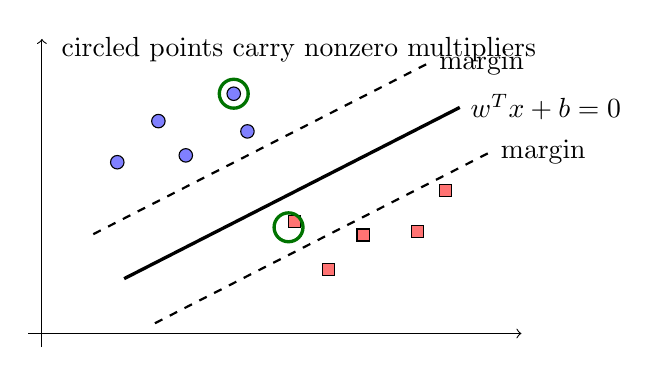
\begin{tikzpicture}[scale=.87]
    \draw[->] (-.2,0)--(7,0);
    \draw[->] (0,-.2)--(0,4.3);
    \draw[very thick] (1.2,.8)--(6.1,3.3) node[right] {$w^Tx+b=0$};
    \draw[thick,dashed] (.75,1.45)--(5.65,3.95) node[right] {margin};
    \draw[thick,dashed] (1.65,.15)--(6.55,2.65) node[right] {margin};
    \foreach \x/\y in {1.1/2.5,1.7/3.1,2.1/2.6,2.8/3.5,3.0/2.95}
      {\draw[fill=blue!50] (\x,\y) circle (2.8pt);}
    \foreach \x/\y in {4.1/.85,4.6/1.35,5.4/1.4,5.8/2.0,3.6/1.55}
      {\draw[fill=red!55] (\x,\y) rectangle +(5pt,5pt);}
    \draw[green!45!black,very thick] (2.8,3.5) circle (6pt);
    \draw[green!45!black,very thick] (3.6,1.55) circle (6pt);
    \node at (3.75,4.15) {circled points carry nonzero multipliers};
  \end{tikzpicture}
  \end{center}
\end{frame}

\begin{frame}{Example 6: mean-variance portfolio with no shorting}
  \[
    \min_w \frac12 w^T\Sigma w
    \quad\text{s.t.}\quad \mathbf{1}^Tw=1,
    \quad r^Tw\ge \rho,
    \quad w_i\ge0.
  \]
  KKT conditions combine three effects:
  \begin{align*}
    &\Sigma w+\nu\mathbf{1}-\eta r-\gamma=0,\\
    &\mathbf{1}^Tw=1,
      \qquad r^Tw\ge\rho,
      \qquad w_i\ge0,\\
    &\eta\ge0,
      \qquad \gamma_i\ge0,
      \qquad \eta(r^Tw-\rho)=0,
      \qquad \gamma_iw_i=0.
  \end{align*}
  \vspace{.2em}
  \begin{itemize}
    \item $\nu$ prices the budget equality.
    \item $\eta$ prices the target return constraint.
    \item $\gamma_i$ prices the no-shorting bound on asset $i$.
  \end{itemize}
\end{frame}

\begin{frame}{How to solve with KKT in practice}
  \begin{enumerate}
    \item Write all constraints in the chosen sign convention.
    \item Form the Lagrangian.
    \item Write stationarity, feasibility, sign, and complementarity equations.
    \item Guess or infer the active set.
    \item Solve the equality system for that active set.
    \item Check feasibility, signs, and complementarity.
  \end{enumerate}
  \vspace{.5em}
  For convex problems, a checked KKT point is a certificate of global optimality.
\end{frame}

\begin{frame}{Common pitfalls}
  \begin{itemize}
    \item Sign convention errors: $g_i(x)\le0$ gives $\lambda_i\ge0$ for minimization.
    \item Forgetting inactive constraints: their multipliers must be zero.
    \item Treating KKT as sufficient in nonconvex problems: it may only be necessary.
    \item Missing constraint qualification: multipliers might fail to exist at singular points.
  \end{itemize}
  \vspace{.6em}
  \begin{block}{Practical mantra}
    KKT is a local first-order balance law. Convexity upgrades that balance into a global certificate.
  \end{block}
\end{frame}

\begin{frame}{Takeaways}
  \begin{center}
  \Large
  KKT conditions describe optimality as a balance of objective gradient and active constraint normals.
  \end{center}
  \vspace{.7em}
  \begin{columns}[T,totalwidth=\textwidth]
  \begin{column}{.32\textwidth}
    \begin{block}{Necessary}
      Local minimizer plus constraint qualification implies KKT.
    \end{block}
  \end{column}
  \begin{column}{.32\textwidth}
    \begin{block}{Sufficient}
      Convex objective and constraints make KKT a global certificate.
    \end{block}
  \end{column}
  \begin{column}{.32\textwidth}
    \begin{block}{Useful}
      Multipliers explain sensitivity and active constraints.
    \end{block}
  \end{column}
  \end{columns}
\end{frame}

\end{document}
